% Guide de paramétrage de StageCompagnon (mod_stage et mod_stagesynthesis).
% Compilation : latexmk -pdf guide-parametrage.tex (deux passes pdflatex suffisent sinon).
\documentclass[11pt,a4paper]{article}

\usepackage[T1]{fontenc}
\usepackage[utf8]{inputenc}
\usepackage{lmodern}
\usepackage[french]{babel}
\usepackage[margin=2.2cm,headheight=14pt]{geometry}
\usepackage{microtype}
\usepackage{amssymb}
\usepackage{graphicx}
\usepackage{float}
\usepackage[font=small,labelfont=bf]{caption}
\usepackage{xcolor}
\usepackage{booktabs}
\usepackage{tabularx}
\usepackage{enumitem}
\usepackage{fancyhdr}
\usepackage[most]{tcolorbox}
\usepackage[hidelinks]{hyperref}

\definecolor{moodle}{HTML}{0F6CBF}
\definecolor{cadre}{HTML}{B0B7BF}

\hypersetup{
  pdftitle={StageCompagnon -- Guide de paramétrage},
  pdfauthor={Sébastien Lefebvre},
  colorlinks=true, linkcolor=moodle, urlcolor=moodle
}

\pagestyle{fancy}
\fancyhf{}
\lhead{\small StageCompagnon -- Guide de paramétrage}
\rhead{\small\nouppercase{\leftmark}}
\cfoot{\small\thepage}

\setlist{itemsep=2pt, topsep=4pt}
\setlength{\parskip}{4pt}
\setlength{\parindent}{0pt}
\setlength{\emergencystretch}{2em}

% Capture d'écran encadrée, numérotée et référencée par fig:<fichier>.
% \capture[largeur]{fichier}{légende}
\newcommand{\capture}[3][\linewidth]{%
  \begin{figure}[H]
    \centering
    \setlength{\fboxsep}{0pt}%
    \fcolorbox{cadre}{white}{\includegraphics[width=\dimexpr#1-2\fboxrule\relax,height=0.70\textheight,keepaspectratio]{images/#2}}
    \caption{#3}
    \label{fig:#2}
  \end{figure}}

% Chemin de navigation dans l'interface : \chemin{Administration > Gérer les thématiques}
\newcommand{\chemin}[1]{\textsf{\textbf{\color{moodle}#1}}}
% Bouton ou libellé d'interface
\newcommand{\bouton}[1]{\textsf{«~#1~»}}

\newtcolorbox{astuce}{colback=moodle!5, colframe=moodle, fonttitle=\bfseries,
  title=À noter, boxrule=0.6pt, arc=2pt}
\newtcolorbox{attention}{colback=orange!6, colframe=orange!80!black, fonttitle=\bfseries,
  title=Attention, boxrule=0.6pt, arc=2pt}
% Texte de courriel : \begin{courriel}{Sujet}...\end{courriel}
\newtcolorbox{courriel}[1]{colback=black!3, colframe=black!40, boxrule=0.4pt, arc=1pt,
  fonttitle=\small\sffamily, coltitle=black, colbacktitle=black!10, title={Sujet : #1},
  fontupper=\small\sffamily, left=6pt, right=6pt}
% Variable de courriel : \var{student} donne {{student}}
\newcommand{\var}[1]{\texttt{\{\{#1\}\}}}

\begin{document}

\begin{titlepage}
  \centering
  \vspace*{3cm}
  {\Huge\bfseries StageCompagnon\par}
  \vspace{0.6cm}
  {\LARGE Guide de paramétrage\par}
  \vspace{0.4cm}
  {\large Modules Moodle \og Gestion des stages\fg{} (\texttt{mod\_stage})\\
   et \og Suivi des stages\fg{} (\texttt{mod\_stagesynthesis})\par}
  \vspace{1.5cm}
  \setlength{\fboxsep}{0pt}
  \fcolorbox{cadre}{white}{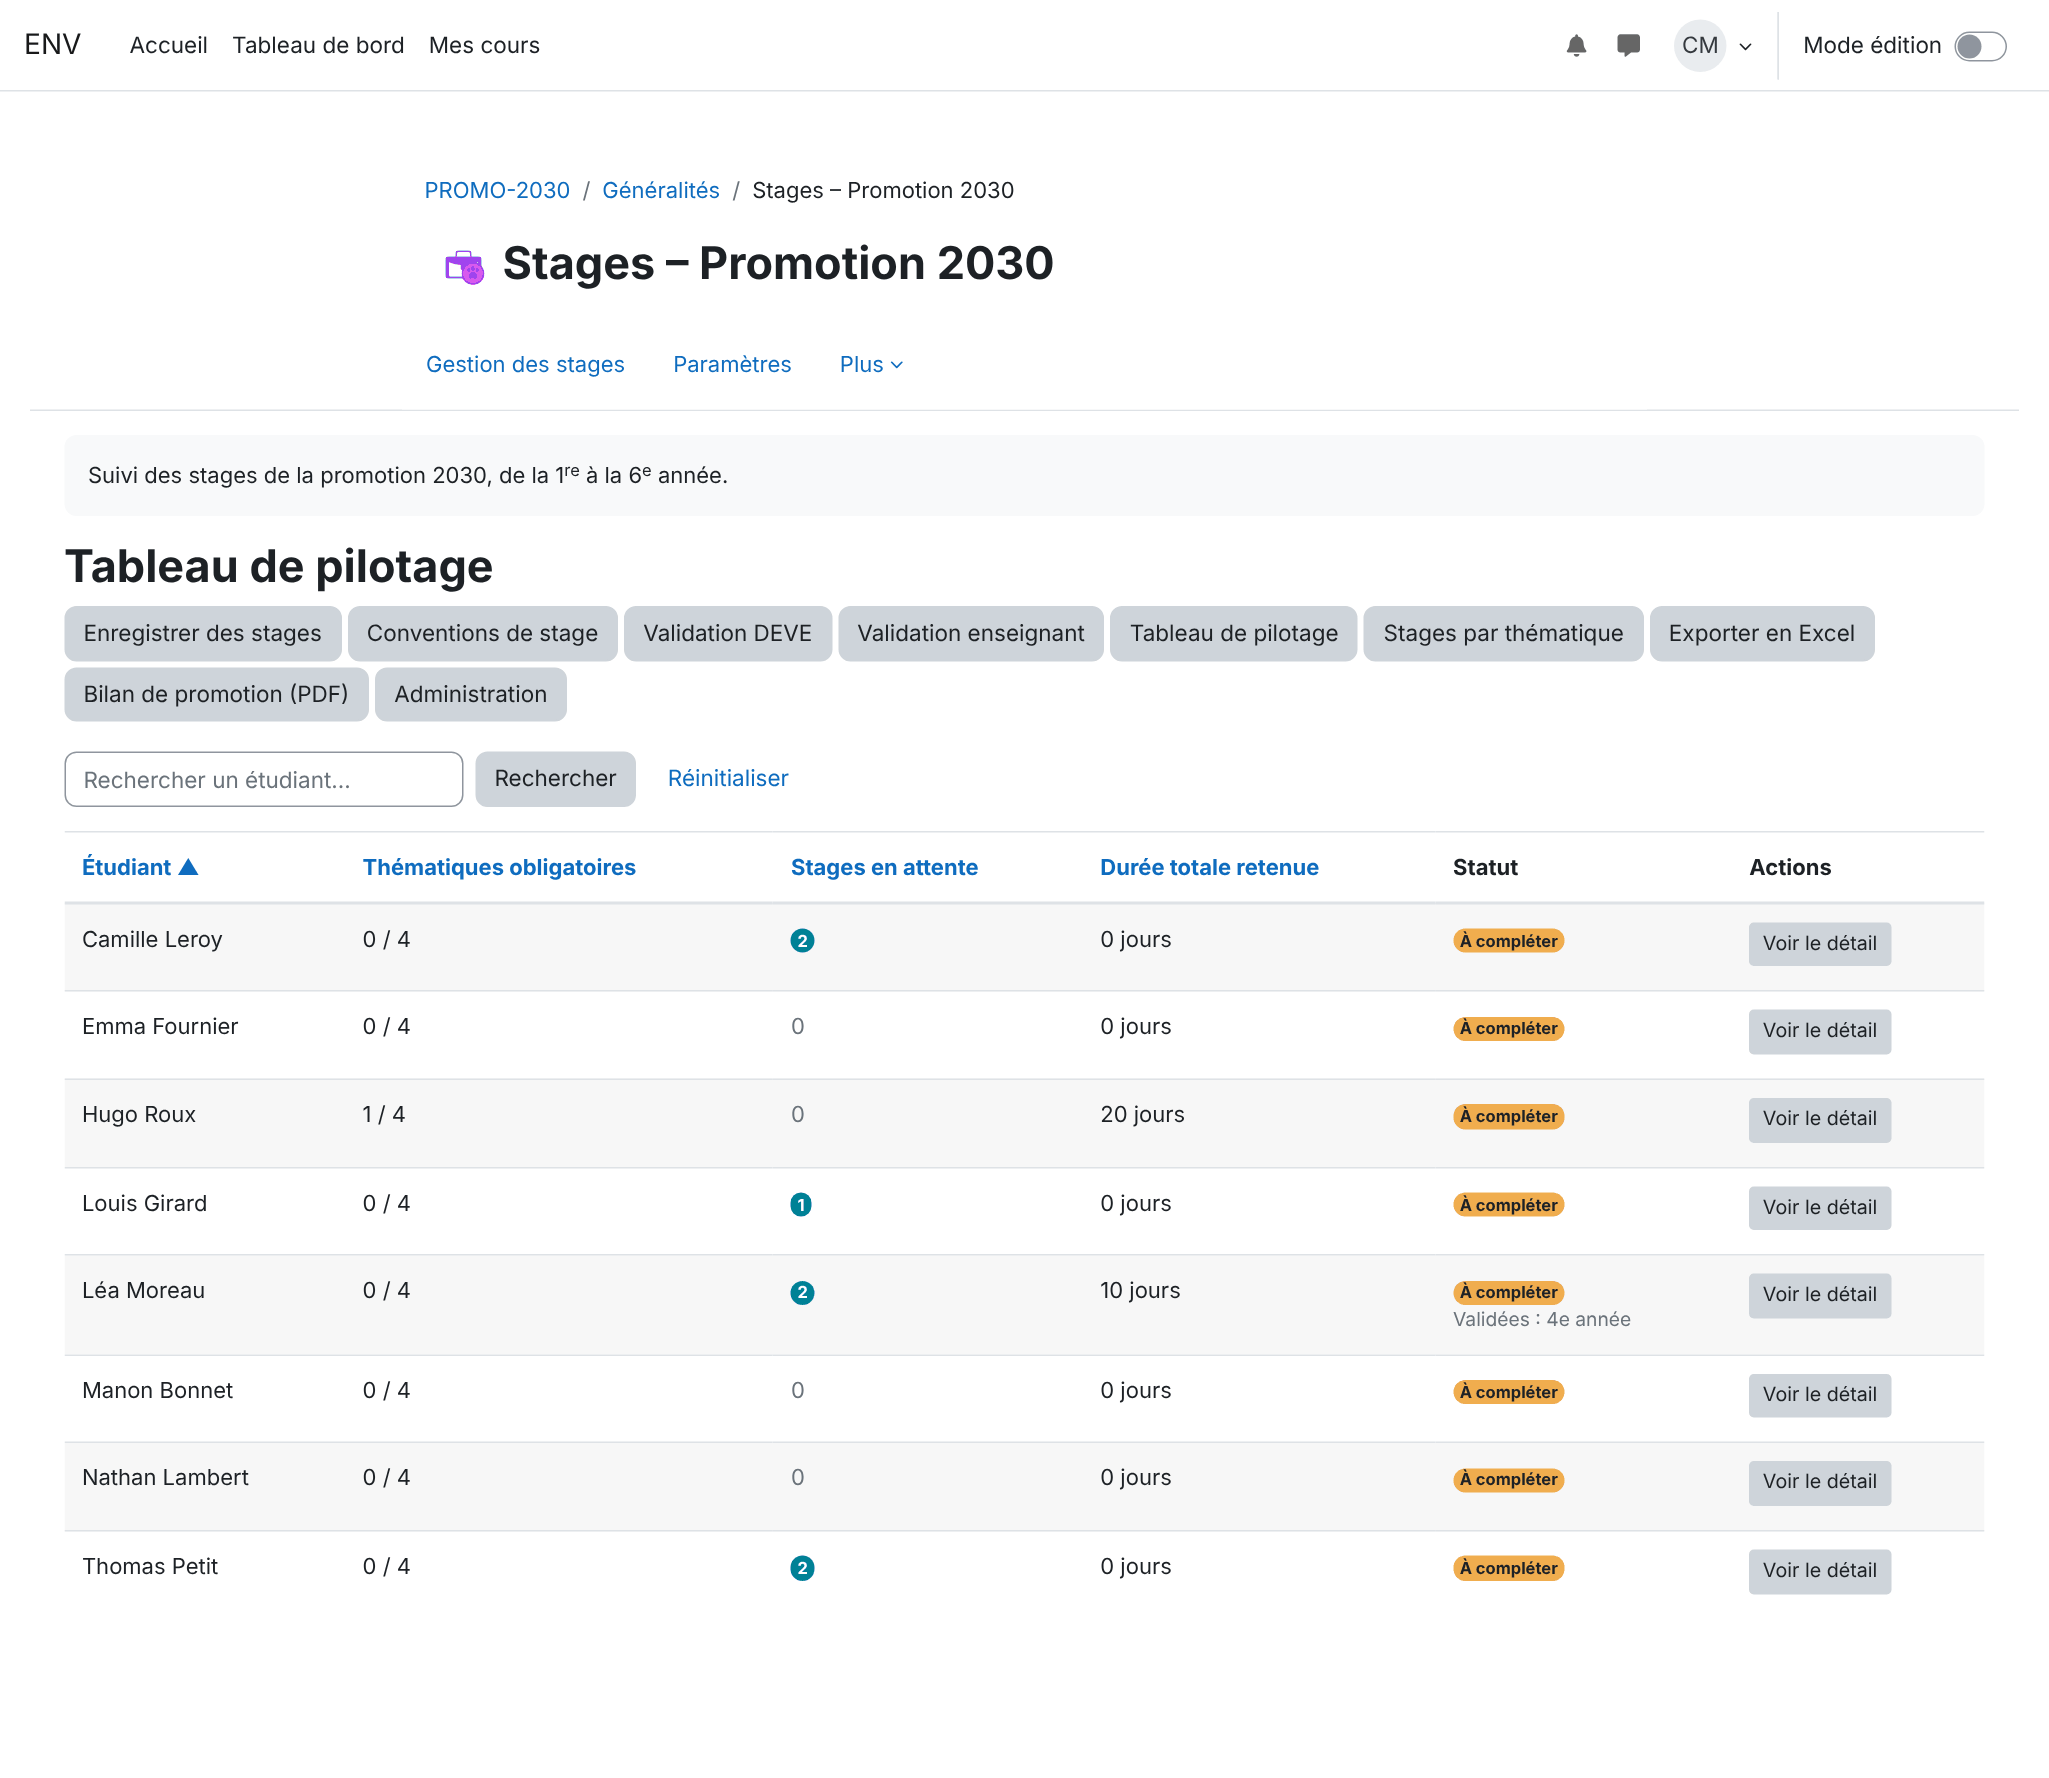
\includegraphics[width=0.85\linewidth]{images/18_dashboard}}
  \vfill
  {\large Sébastien Lefebvre\par}
  {\large \today\par}
\end{titlepage}

\tableofcontents
\newpage

% ===========================================================================
\section{Principe d'organisation}

\subsection{Un cours par promotion}

Chaque promotion a son propre cours, nommé d'après elle :
\og Stages -- Promotion 2030\fg{}, \og Stages -- Promotion 2031\fg{}, etc.
Le cours suit les mêmes étudiants de la 1\textsuperscript{re} à la
6\textsuperscript{e}~année. Tous leurs stages y restent, ce qui permet d'en
faire le bilan sur l'ensemble du cursus.

Trois réglages et actions découlent de ce choix :
\begin{itemize}
  \item l'activité indique l'\textbf{année d'étude} où se trouve la promotion ;
        elle est mise à jour à chaque rentrée ;
  \item un étudiant qui \textbf{redouble} quitte sa promotion : ses stages sont
        transférés dans le cours de la promotion qu'il rejoint ;
  \item une \textbf{nouvelle promotion} reprend le paramétrage de la précédente
        par import.
\end{itemize}

\subsection{Les trois cas}

\begin{center}
\begin{tabularx}{\linewidth}{@{}l l X@{}}
\toprule
\textbf{Cas} & \textbf{Quand} & \textbf{Ce qu'on fait} \\
\midrule
Mise en place (§\ref{sec:cas1}) & Arrivée d'une promotion & Créer le cours, importer ou saisir le paramétrage, inscrire, attribuer les référents \\
Rentrée (§\ref{sec:cas2}) & Chaque année & Passer l'activité à l'année suivante, vérifier les référents \\
Redoublement (§\ref{sec:cas3}) & Fin d'année, avant la rentrée & Transférer l'étudiant et ses stages vers la promotion suivante \\
\bottomrule
\end{tabularx}
\end{center}

La partie \ref{sec:courriels} détaille les courriels : textes standard,
variables et exemples de personnalisation.

\subsection{Rôles}

Le module utilise les rôles standard de Moodle. Ne créez pas de rôle
\og DEVE\fg{}.

\begin{center}
\begin{tabularx}{\linewidth}{@{}l l X@{}}
\toprule
\textbf{Rôle Moodle} & \textbf{Fonction} & \textbf{Intervient sur} \\
\midrule
Administrateur & Administration du site & Installation, services web \\
Enseignant & DEVE & Paramétrage, transferts, validation finale \\
Enseignant non éditeur & Enseignant référent & Validation des conventions, évaluation \\
Étudiant & Étudiant & Demande de convention, auto-évaluation \\
Aucun compte & Maître de stage & Évaluation par lien à usage unique \\
\bottomrule
\end{tabularx}
\end{center}

Les captures proviennent d'un Moodle~4.5 de démonstration (personnes et
structures fictives). Claire Martin y est la DEVE, Paul Durand et Julie Bernard
sont référents. Quelques libellés propres à Moodle sont restés en anglais ; sur
votre plateforme, ils suivent la langue installée.

% ===========================================================================
\section{Cas 1 : mise en place d'une promotion}
\label{sec:cas1}

\subsection{Installer les modules (une seule fois)}
\label{sec:installation}

\begin{verbatim}
cp -r mod/stage           <moodle>/mod/stage
cp -r mod/stagesynthesis  <moodle>/mod/stagesynthesis   # facultatif
php admin/cli/upgrade.php
\end{verbatim}

Sans accès à la ligne de commande, connectez-vous en administrateur : Moodle
propose l'installation. Prérequis : Moodle~4.0, PHP~7.4.
\texttt{mod\_stagesynthesis} nécessite \texttt{mod\_stage}.

\capture{01_plugins}{Les deux modules installés
(\chemin{Administration du site > Plugins > Activités}).}

\subsection{Créer le cours et inscrire les participants}

Créez le cours \og Stages -- Promotion 2030\fg{}, puis inscrivez :
\begin{itemize}
  \item les étudiants de la promotion avec le rôle \bouton{Étudiant} ;
  \item les référents avec le rôle \bouton{Enseignant non éditeur} ;
  \item la DEVE avec le rôle \bouton{Enseignant}.
\end{itemize}

\capture{02c_participants}{Participants du cours de la promotion.}

\begin{attention}
Le rôle \og Enseignant\fg{} donne tous les droits DEVE. Réservez-le à la
scolarité.
\end{attention}

\subsection{Ajouter l'activité et indiquer l'année d'étude}
\label{sec:annee}

En mode édition : \chemin{Ajouter une activité ou ressource > Gestion des
stages}. Renseignez :
\begin{itemize}
  \item le \textbf{nom}, par exemple \og Stages -- Promotion 2030\fg{}. Ce nom
        apparaît dans les courriels envoyés (variable \var{stage},
        §\ref{sec:variables}) : choisissez un nom compréhensible hors de Moodle ;
  \item l'\textbf{année d'étude courante des étudiants} : l'année où se trouve
        la promotion aujourd'hui.
\end{itemize}

\capture{02_add_stage}{Création de l'activité de la promotion 2030, actuellement
en 5\textsuperscript{e}~année.}

L'année d'étude courante, notée \(N\), a trois effets :
\begin{itemize}
  \item un étudiant qui déclare lui-même un stage ne peut le rattacher qu'aux
        années \(N-1\), \(N\) ou \(N+1\) ;
  \item le bilan d'un étudiant (sa page \og Mes stages\fg{} et le détail vu par
        la DEVE et le référent) n'affiche que les années \(1\) à \(N\) ;
  \item le bilan de promotion (PDF et export Excel) ne retient que les années
        \(1\) à \(N\).
\end{itemize}
Avec \og Non spécifiée\fg{}, toutes les années sont proposées et affichées.

\capture[0.8\linewidth]{02b_course}{L'activité dans le cours de la promotion.}

\subsection{Reprendre le paramétrage d'une autre promotion}
\label{sec:import-cours}

Si une promotion existe déjà, son paramétrage se recopie en une fois. Depuis la
nouvelle activité (ici \og Promotion 2031\fg{}) :
\chemin{Administration > Importer depuis un autre cours}.

\capture{13_admin_import}{Choix de l'activité source et des éléments à copier.}

\begin{center}
\begin{tabularx}{\linewidth}{@{}X l@{}}
\toprule
\textbf{Élément} & \textbf{Effet} \\
\midrule
Thématiques, avec durées, objectifs et listes d'évaluation & Ajoutées (pas de doublon de nom) \\
Gabarits de convention & Ajoutés (pas de doublon de nom) \\
Logos & Remplacés \\
Textes des courriels personnalisés & Remplacés \\
Informations de l'établissement & Remplacées \\
\midrule
Année d'étude courante & \textbf{Non copiée} \\
Durées totales par année, mobilité internationale & \textbf{Non copiées} \\
Référents, stages & \textbf{Non copiés} \\
\bottomrule
\end{tabularx}
\end{center}

\capture{13c_import_done}{Compte rendu de l'import.}

Après l'import, saisissez les durées par année et la mobilité
(§\ref{sec:durees}), puis passez directement aux référents
(§\ref{sec:referents}). Sans promotion source, paramétrez les éléments un par un
(§\ref{sec:thematiques} à §\ref{sec:notifs}).

\subsection{La page Administration}

À l'ouverture de l'activité, la DEVE arrive sur le tableau de pilotage. Le bouton
\bouton{Administration} donne accès au paramétrage.

\capture{03_administration}{La page Administration.}

\subsection{Thématiques}
\label{sec:thematiques}

Une thématique est un type de stage. Elle fixe la durée exigée, les années
concernées, les objectifs et les questionnaires.
\chemin{Administration > Gérer les thématiques}.

\capture{04_themes}{Liste des thématiques.}

Le tableau se modifie en une seule fois : années minimum et maximum, caractère
obligatoire, évaluation par le maître de stage, rapport de stage. La colonne
\og Visible\fg{} retire une thématique des nouveaux enregistrements sans toucher
aux stages existants.

Un clic sur le nom ouvre la fiche de la thématique, enregistrée en une fois.

\capture{05a_theme_top}{Paramètres généraux d'une thématique.}

\paragraph{Durée requise.} Une durée unique, ou une durée par année. Une année
laissée vide reprend la durée unique.

\capture[0.85\linewidth]{05b_theme_durations}{Durée requise.}

\paragraph{Enseignants responsables.} Ils voient les stages de la thématique et
les rapports déposés.

\capture[0.85\linewidth]{05c_theme_teachers}{Enseignants responsables.}

\paragraph{Objectifs.} Les documents déposés sont téléchargeables par
l'étudiant, les enseignants et le maître de stage. La check-list est remplie par
l'étudiant lors de sa demande de convention ; tout objectif non coché doit être
justifié.

\capture[0.85\linewidth]{05d_theme_objectives}{Documents d'objectifs.}
\capture[0.85\linewidth]{05e_theme_checklist}{Check-list d'objectifs.}

\paragraph{Listes d'évaluation.} Une liste par formulaire : étudiant, référent,
maître de stage. Sans liste, le formulaire se limite à un commentaire libre.

\capture[0.85\linewidth]{05f_theme_lists}{Choix des listes d'évaluation.}

\subsection{Durées par année et mobilité internationale}
\label{sec:durees}

\chemin{Administration > Durées totales requises par année} : durée totale
exigée pour chaque année (hors stages complémentaires), jours de stage à
l'étranger, année avant laquelle ils sont dus et consigne affichée aux
étudiants.

\capture{06_year_requirements}{60~jours en 5\textsuperscript{e}~année ; 20~jours
à l'étranger avant la 5\textsuperscript{e}~année.}

\subsection{Listes d'évaluation}

\chemin{Administration > Listes d'évaluation}. Le formulaire de destination
d'une liste est fixé à sa création. Questions à choix multiples (une option par
ligne) ou en texte libre ; une ligne vide ajoute une question. Les questions du
maître de stage ont une version anglaise.

\capture{07_evallists}{Listes d'évaluation.}
\capture{08_evallist_edit}{Liste destinée au maître de stage.}

\begin{attention}
Une question partagée entre plusieurs listes se modifie partout. Retirer une
question présente dans aucune autre liste la supprime avec ses réponses.
\end{attention}

\subsection{Conventions}
\label{sec:conventions}

\chemin{Administration > Gabarits de convention}.

Un gabarit est le PDF des articles juridiques, ajouté après la première page
générée par le module. L'étudiant le choisit lors de sa demande. Un gabarit
utilisé ne peut plus être supprimé.

\capture{09a_templates_list}{Gabarits et nombre de demandes associées.}
\capture[0.85\linewidth]{10_convention_template}{Fiche d'un gabarit.}

L'option \bouton{Exiger la validation de l'enseignant.e référent.e avant
transmission à la DEVE} fait passer chaque demande étudiante par le référent.

\capture[0.85\linewidth]{09b_templates_settings}{Validation par le référent.}

Les informations de l'établissement et deux logos PNG figurent en tête de chaque
convention.

\capture[0.85\linewidth]{09c_templates_establishment}{Établissement.}
\capture[0.85\linewidth]{09d_templates_logos}{Logos.}

\subsection{Notifications et courriels}
\label{sec:notifs}

\chemin{Administration > Notifications et e-mails}. La case \bouton{Activer
l'évaluation par le maître de stage} déclenche l'invitation du maître de stage
(§\ref{sec:liste-courriels}). Les textes des courriels se personnalisent sur la
même page : voir la partie~\ref{sec:courriels}.

\capture{12_notifications}{Notifications et courriels.}

\subsection{Enseignants référents}
\label{sec:referents}

\chemin{Administration > Attribuer les enseignants référents}. Un étudiant sans
référent ne peut pas demander de convention.

\capture{11_teachers}{Attribution des référents. Nathan Lambert n'en a pas.}

Choix ligne par ligne, filtre \bouton{Étudiants sans référent uniquement},
action en masse (ajouter, remplacer, retirer), ou import CSV
\texttt{studentemail;teacher1email;teacher2email}.

\subsection{Enregistrer les stages existants}
\label{sec:enregistrement}

\chemin{Enregistrer des stages}.

\begin{center}
\begin{tabularx}{\linewidth}{@{}X l@{}}
\toprule
\textbf{Méthode} & \textbf{Convention au départ} \\
\midrule
Un stage pour un étudiant & Non demandée \\
Une thématique pour plusieurs étudiants & Signée (StageVet) \\
Fichier CSV & Non demandée \\
Export StageVet & Signée (StageVet) \\
\bottomrule
\end{tabularx}
\end{center}

\capture{14_register}{Stages enregistrés et voies d'enregistrement.}

Colonnes du CSV :
\begin{center}
\texttt{email;theme;structure;datestart;dateend;duration;studyyear}
\end{center}
Dates au format \texttt{AAAA-MM-JJ} ou \texttt{JJ/MM/AAAA}. En-tête facultatif.

\capture{15_import}{Import CSV.}

\subsection{Tester le circuit}
\label{sec:verification}

Suivez un stage avec un compte de chaque rôle.

\paragraph{Étudiant.} La page \og Mes stages\fg{} présente son bilan par année,
ses thématiques obligatoires, la mobilité et ses stages. Pour un stage
enregistré, il dépose sa demande de convention.

\capture{20_student}{Page \og Mes stages\fg{}.}
\capture{20b_student_stages}{Stages et statut des conventions.}
\capture{27_convention_request}{Demande de convention (début).}

\paragraph{Référent.} Les demandes à valider apparaissent en tête de
\chemin{Validation enseignant}, au-dessus des stages à évaluer.

\capture{19_teacher}{Page \og Validation enseignant\fg{}.}
\capture{26_teacher_validate}{Validation d'une demande par le référent.}

\paragraph{DEVE.} \chemin{Conventions de stage} :
\bouton{Générer la convention} ouvre la demande ; \bouton{Valider} produit le
PDF, \bouton{Refuser} la renvoie à l'étudiant ; \bouton{Marquer signée} ouvre
l'auto-évaluation.

\capture{16_conventions}{Suivi des conventions.}
\capture{25a_review_top}{Demande ouverte pour génération.}
\capture{25b_review_generate}{Cadre de signatures pour un exemplaire papier.}

\chemin{Validation DEVE} : validation unitaire ou en masse, refus,
réinitialisation. Le \chemin{Tableau de pilotage} résume la promotion.

\capture{17_deve}{Validation DEVE.}
\capture{29_deve_validate}{Validation d'un stage.}
\capture{18_dashboard}{Tableau de pilotage.}

\subsection{Lier la promotion au suivi multi-promotions}

Le module \og Suivi des stages\fg{} regroupe, pour chaque référent, ses étudiants
de toutes les promotions. Il ne stocke aucune donnée.

\begin{enumerate}
  \item Une seule fois : créer un cours \og Suivi des référents de stage\fg{},
        y inscrire les référents et ajouter une activité \bouton{Suivi des
        stages}.
  \item Pour chaque nouvelle promotion : dans \chemin{Gérer les liens}, cocher
        son activité.
\end{enumerate}

\capture{21_add_synthesis}{Création de l'activité \og Suivi des stages\fg{}.}
\capture{22_synth_links}{Activités liées : la promotion 2031 reste à cocher.}
\capture{23_synth_view}{Pilotage multi-promotions d'un référent.}
\capture{24_synth_entries}{Demandes à valider et stages à évaluer.}

% ===========================================================================
\section{Cas 2 : à chaque rentrée}
\label{sec:cas2}

Pour chaque promotion en cours :
\begin{enumerate}
  \item \textbf{Traiter d'abord les redoublants} (§\ref{sec:cas3}), tant que
        l'année d'étude n'a pas changé.
  \item \textbf{Passer à l'année suivante} : dans l'activité,
        \chemin{Paramètres > Année d'étude courante des étudiants}, augmenter
        d'une année (par exemple de \og 4e année\fg{} à \og 5e année\fg{}).
  \item \textbf{Vérifier les référents} (§\ref{sec:referents}) si l'équipe
        change.
  \item \textbf{Vérifier les durées} de la nouvelle année
        (§\ref{sec:durees}) si les exigences ont évolué.
\end{enumerate}
Pour la promotion qui arrive, appliquer le cas~1, en important le paramétrage
d'une promotion existante.

\capture{34_update_year}{Paramètres de l'activité de la promotion 2031 : l'année
passe ici de 4\textsuperscript{e} à 5\textsuperscript{e}~année.}

\begin{attention}
L'année ne change jamais d'elle-même, et la réinitialisation du cours ne la
modifie pas. Ne réinitialisez pas le cours d'une promotion : elle supprimerait les
stages et les attributions de référents des années précédentes.
\end{attention}

% ===========================================================================
\section{Cas 3 : un étudiant redouble}
\label{sec:cas3}

L'étudiant quitte sa promotion pour la suivante. Ses stages \textbf{sont
déplacés}, pas copiés : son bilan le suit et disparaît du cours de départ.
Exemple : Emma Fournier quitte la promotion 2030 pour la promotion 2031.

\paragraph{1. Préparer la promotion d'accueil.} Son activité doit contenir les
mêmes thématiques, avec exactement les mêmes noms. Si elle a été créée par
import (§\ref{sec:import-cours}), c'est déjà le cas.

\paragraph{2. Inscrire l'étudiant} dans le cours de la promotion d'accueil, avec
le rôle \bouton{Étudiant}. Le transfert est refusé sans cette inscription.

\paragraph{3. Transférer.} Depuis l'activité de départ :
\chemin{Administration > Transférer un étudiant}. Choisir l'étudiant et
l'activité de destination, puis \bouton{Préparer le transfert}.

\capture{31_transfer_form}{Choix de l'étudiant et de la promotion d'accueil.}

Le récapitulatif liste les stages déplacés et signale ce qui bloque ou se perd.

\capture{32_transfer_preview}{Récapitulatif avant confirmation.}

\begin{center}
\begin{tabularx}{\linewidth}{@{}l X@{}}
\toprule
\textbf{Message} & \textbf{Action} \\
\midrule
Aucun stage dans l'activité de départ & Rien à transférer \\
Étudiant non inscrit & Bloquant : l'inscrire (étape 2) \\
Thématique absente & Bloquant : la créer avec le même nom, ou importer \\
Objectif de check-list sans correspondance & Bloquant : ajouter l'objectif dans la thématique cible \\
Gabarit de convention absent & Stage transféré sans gabarit ; la convention signée reste disponible \\
Réponses sans question correspondante & Ces réponses seront supprimées \\
Référents non transférés & À attribuer dans la promotion d'accueil (étape 4) \\
\bottomrule
\end{tabularx}
\end{center}

\bouton{Confirmer le transfert}. L'opération n'est pas réversible d'un clic : il
faudrait refaire un transfert en sens inverse.

\capture{33_transfer_done}{Confirmation du transfert.}

\paragraph{4. Finaliser dans la promotion d'accueil.} Vérifier que les stages
sont arrivés, puis attribuer un référent.

\capture{35_target_entries}{Les stages d'Emma Fournier dans la promotion 2031.}
\capture{36_target_teachers}{Emma Fournier est \og Sans référent\fg{} : à attribuer.}

\paragraph{5. Désinscrire l'étudiant du cours de départ.} Sinon il reste dans le
tableau de pilotage de son ancienne promotion, sans stage.

Les stages gardent l'année d'étude à laquelle ils ont été rattachés. Le même
transfert sert pour un changement de promotion ou une réorientation vers un autre
cours.

% ===========================================================================
\section{Courriels}
\label{sec:courriels}

\subsection{Fonctionnement}

\begin{itemize}
  \item Les courriels partent en texte brut, depuis l'adresse \og no-reply\fg{}
        du site Moodle.
  \item Chaque activité a ses propres textes. Un texte personnalisé remplace le
        texte standard ; laisser le sujet \emph{et} le corps vides rétablit le
        texte standard. On peut ne personnaliser que le sujet, ou que le corps.
  \item Les variables s'écrivent entre doubles accolades, par exemple
        \var{student}. Seules les variables listées sous chaque formulaire sont
        remplacées.
  \item Les textes personnalisés se recopient vers une autre promotion avec
        l'import (option \og Textes des courriels\fg{}).
\end{itemize}

\capture[0.85\linewidth]{12b_notification_open}{Courriel non personnalisé : champs
vides et variables disponibles.}

\subsection{Liste des courriels}
\label{sec:liste-courriels}

\begin{center}
\small
\begin{tabularx}{\linewidth}{@{}>{\raggedright\arraybackslash}p{3.6cm} l X@{}}
\toprule
\textbf{Courriel} & \textbf{À} & \textbf{Envoyé quand} \\
\midrule
Auto-évaluation & Référents & L'étudiant soumet son auto-évaluation. \\
Convention à valider & Référents & L'étudiant dépose une demande et la validation par le référent est activée. \\
Convention refusée & Étudiant & Le référent ou la DEVE refuse la demande. \\
Convention prête & Étudiant & La DEVE génère la convention avec le cadre de signatures (à chaque génération). \\
Invitation du maître de stage & Maître de stage & Tâche quotidienne (6~h~45), à partir du premier jour du stage, une seule fois, si l'option est active pour l'activité et la thématique, la convention signée ou dispensée, et le courriel du maître de stage renseigné. \\
Demande d'évaluation après import & Référents & Un import StageVet réunit les évaluations de l'étudiant et du maître de stage. \\
Rappel de convention non signée & Étudiant & Tâche quotidienne (6~h~30), une seule fois, quand le stage commence dans 7~jours ou moins sans convention signée. \\
\bottomrule
\end{tabularx}
\end{center}

\subsection{Variables}
\label{sec:variables}

\begin{center}
\begin{tabularx}{\linewidth}{@{}l X l@{}}
\toprule
\textbf{Variable} & \textbf{Valeur} & \textbf{Exemple} \\
\midrule
\var{student} & Prénom et nom de l'étudiant & Emma Fournier \\
\var{stage} & Nom de l'\emph{activité} (pas du lieu de stage) & Stages -- Promotion 2030 \\
\var{theme} & Thématique du stage & Équine \\
\var{url} & Lien vers la page à ouvrir (voir ci-dessous) & \\
\var{comment} & Motif du refus & Dates manquantes \\
\var{datestart} & Date de début du stage & 2 novembre 2026 \\
\var{days} & Délai du rappel, en jours & 7 \\
\bottomrule
\end{tabularx}
\end{center}

Le lien \var{url} ouvre l'évaluation du stage (référents), la page
\og Validation enseignant\fg{} (convention à valider), le formulaire de demande
(refus, rappel), la page \og Mes stages\fg{} (convention prête) ou le
questionnaire sans compte (maître de stage).

\subsection{Textes standard}

Textes envoyés tant qu'aucune personnalisation n'est enregistrée. Les valeurs
entre accolades sont remplacées comme indiqué ci-dessus.

\begin{courriel}{Auto-évaluation de stage à évaluer - \var{stage}}
\var{student} vient de s'auto-évaluer pour son stage "\var{stage}". Vous pouvez
consulter et évaluer cette saisie ici : \var{url}
\end{courriel}

\begin{courriel}{Convention de stage à valider : \var{stage}}
Un.e étudiant.e que vous encadrez a soumis une demande de convention pour le stage
"\var{stage}", qui attend votre validation avant transmission à la DEVE :\\
\var{url}
\end{courriel}

\begin{courriel}{Convention de stage refusée : \var{stage}}
Votre demande de convention pour le stage "\var{stage}" a été refusée par la DEVE,
pour le motif suivant :\\[4pt]
\var{comment}\\[4pt]
Merci de corriger votre demande et de la soumettre à nouveau :\\
\var{url}
\end{courriel}

\begin{courriel}{Votre convention de stage est disponible : \var{stage}}
Bonjour \var{student},\\[4pt]
Votre convention de stage pour la thématique "\var{theme}" a été éditée par la
scolarité : elle est désormais téléchargeable depuis votre espace de suivi des
stages.\\
\var{url}\\[4pt]
Merci de l'imprimer, de la faire signer par toutes les parties, puis de la
retourner à la scolarité.
\end{courriel}

\begin{courriel}{Évaluation du stage de \var{stage}}
Vous encadrez actuellement \var{student} dans le cadre de son stage
"\var{stage}". Merci de bien vouloir évaluer ce stage en suivant ce lien, qui ne
nécessite pas de compte :\\
\var{url}
\end{courriel}

\begin{courriel}{Stage à évaluer - \var{stage}}
Les évaluations de l'étudiant et du maître de stage sont disponibles pour le
stage de \var{student} (thématique « \var{theme} », \var{stage}). Merci de
procéder à votre évaluation : \var{url}
\end{courriel}

\begin{courriel}{Convention de stage non signée : \var{stage}}
Bonjour \var{student},\\[4pt]
Votre stage "\var{theme}" commence le \var{datestart}, soit dans moins de
\var{days} jours, et sa convention n'est toujours pas signée. Sans convention
signée, le stage ne peut pas débuter.\\[4pt]
Merci de régulariser votre demande de convention au plus vite :\\
\var{url}
\end{courriel}

Pour l'invitation du maître de stage, le texte standard existe aussi en anglais.
Il est envoyé en anglais quand la convention utilise un gabarit anglais.

\subsection{Points à corriger par la personnalisation}

\begin{itemize}
  \item \var{stage} vaut le nom de l'activité. Le sujet standard de
        l'invitation devient ainsi \og Évaluation du stage de Stages --
        Promotion 2030\fg{}, peu clair pour un maître de stage.
  \item Le refus standard dit \og refusée par la DEVE\fg{}, même quand c'est le
        référent qui refuse.
  \item Aucun texte standard ne donne d'adresse de contact ni de signature.
  \item Un texte personnalisé est envoyé tel quel, \textbf{quelle que soit la
        langue de la convention}. Pour l'invitation du maître de stage, écrivez-le
        en français et en anglais si vous avez des conventions en anglais.
\end{itemize}

\subsection{Exemples}

\subsubsection*{Refus de convention, quel que soit l'auteur.}

\begin{courriel}{Demande de convention à corriger -- \var{stage}}
Bonjour,\\[4pt]
Votre demande de convention n'a pas pu être acceptée en l'état, pour le motif
suivant :\\[4pt]
\var{comment}\\[4pt]
Corrigez-la puis soumettez-la de nouveau depuis cette page :\\
\var{url}\\[4pt]
Le service des stages
\end{courriel}

\capture[0.85\linewidth]{12c_notification_custom}{Le même texte saisi dans
l'activité. La section est marquée \og (personnalisé)\fg{}.}

\subsubsection*{Invitation du maître de stage, bilingue.}

\begin{courriel}{Évaluation du stage de \var{student} / Internship evaluation}
Madame, Monsieur,\\[4pt]
Vous accueillez actuellement \var{student}, étudiant(e) de l'École nationale
vétérinaire. Merci de bien vouloir évaluer son stage à l'aide du lien
ci-dessous (environ 5 minutes, sans création de compte) :\\
\var{url}\\[4pt]
You are currently supervising \var{student}, a student of our veterinary school.
Please evaluate the internship using the link above (about 5 minutes, no
account needed).\\[4pt]
Service des stages -- stages@ecole-veto.fr
\end{courriel}

\subsubsection*{Convention prête, avec les consignes de retour.}

\begin{courriel}{Convention à signer -- \var{theme}}
Bonjour \var{student},\\[4pt]
Votre convention pour le stage \og \var{theme}\fg{} est prête. Téléchargez-la
depuis votre espace :\\
\var{url}\\[4pt]
Faites-la signer par l'organisme d'accueil et votre maître de stage, puis
déposez-la au bureau des stages (bâtiment A, bureau 12) au moins une semaine
avant le début du stage.\\[4pt]
Le service des stages
\end{courriel}

\subsubsection*{Rappel de convention non signée.}

\begin{courriel}{Urgent : convention non signée pour votre stage du \var{datestart}}
Bonjour \var{student},\\[4pt]
Votre stage \og \var{theme}\fg{} commence le \var{datestart} et la convention
n'est pas signée. Sans convention signée, vous ne pouvez pas commencer ce stage
et n'êtes pas assuré(e).\\[4pt]
Faites le point sur votre demande :\\
\var{url}\\[4pt]
Le service des stages -- stages@ecole-veto.fr
\end{courriel}

% ===========================================================================
\section{Services web (facultatif)}
\label{sec:ws}

Le service \og Gestion des stages (mod\_stage)\fg{} expose
\texttt{mod\_stage\_register\_entries} et \texttt{mod\_stage\_get\_my\_stages}.
Activer les services web et REST (\chemin{Administration du site > Serveur >
Services web}), activer le service, y autoriser un compte, générer un jeton.

\capture{30_ws}{Le service dans la liste des services externes.}

% ===========================================================================
\section{Récapitulatif}

\begin{center}
\begin{tabularx}{\linewidth}{@{}c X l@{}}
\toprule
\(\square\) & \textbf{Mise en place d'une promotion} & \textbf{Page} \\
\midrule
\(\square\) & Cours \og Stages -- Promotion AAAA\fg{} créé, participants inscrits & Participants \\
\(\square\) & Activité créée, année d'étude renseignée & Paramètres de l'activité \\
\(\square\) & Paramétrage importé, ou saisi & Importer depuis un autre cours \\
\(\square\) & Durées par année, mobilité & Durées totales requises \\
\(\square\) & Courriels relus ou personnalisés & Notifications et e-mails \\
\(\square\) & Un référent par étudiant & Attribuer les référents \\
\(\square\) & Activité cochée dans le suivi multi-promotions & Gérer les liens \\
\midrule
 & \textbf{Rentrée} & \\
\midrule
\(\square\) & Redoublants transférés & Transférer un étudiant \\
\(\square\) & Année d'étude augmentée d'un an & Paramètres de l'activité \\
\(\square\) & Référents vérifiés & Attribuer les référents \\
\midrule
 & \textbf{Redoublement} & \\
\midrule
\(\square\) & Inscrit dans la promotion d'accueil & Participants \\
\(\square\) & Stages transférés & Transférer un étudiant \\
\(\square\) & Référent attribué dans la promotion d'accueil & Attribuer les référents \\
\(\square\) & Désinscrit du cours de départ & Participants \\
\bottomrule
\end{tabularx}
\end{center}

\end{document}
